% \documentclass[hcross_theory.tex]{subfiles}
\documentclass{standalone}

\usepackage{tikz}
\usetikzlibrary{backgrounds}
\usetikzlibrary{math}
\usepackage{multirow}

\usetikzlibrary{
    positioning, 
    calc, 
    % external, 
    patterns, 
    arrows.meta, 
    shapes.arrows, 
    shapes.misc}
\usepackage{tikz-3dplot}

\begin{document}

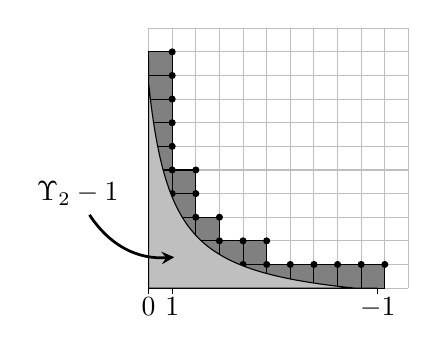
\begin{tikzpicture}[scale=0.3]
\newcommand{\hcrossouterradiustikz}{10.7}
\newcommand{\hcrossinnerradiustikz}{9.7}
\newcommand{\hcrossnxnytikz}{11}

\draw[lightgray] (0,0) grid (\hcrossnxnytikz,\hcrossnxnytikz);

\foreach \x in {0,1,...,\hcrossnxnytikz}
{
\foreach \y in {0,1,...,\hcrossnxnytikz}
{
\pgfmathsetmacro{\Jn}{ifthenelse(\x*\y<=\hcrossouterradiustikz,ifthenelse(\x<=\hcrossouterradiustikz,ifthenelse(\y<=\hcrossouterradiustikz,ifthenelse(\x>0,ifthenelse(\y>0,1,0),0),0),0),0)}
\ifthenelse{\Jn=1}
{
    \path [fill=gray,draw=black] (\x-1.0,\y-1.0) rectangle (\x-0.0,\y-0.0);
}
{}
}
}

\foreach \x in {0,1,...,\hcrossnxnytikz}
{
\foreach \y in {0,1,...,\hcrossnxnytikz}
{
\pgfmathsetmacro{\Jn}{ifthenelse(\x*\y<=\hcrossouterradiustikz,ifthenelse(\x<=\hcrossouterradiustikz,ifthenelse(\y<=\hcrossouterradiustikz,ifthenelse(\x>0,ifthenelse(\y>0,1,0),0),0),0),0)}
\ifthenelse{\Jn=1}
{
    \node[draw,circle,inner sep=0.75pt,fill,color=black] at (\x,\y) {};
}
{}
}
}

\draw[fill=gray!50] plot[smooth, samples=100, domain=1:\hcrossinnerradiustikz] (\x-1, \hcrossinnerradiustikz / \x - 1) -- (\hcrossinnerradiustikz,0) -- (0,0) -- (0,\hcrossinnerradiustikz) -- cycle;

\draw (0,0)--(0,-.25);

\draw (1,0)--(1,-.25);

\draw (\hcrossinnerradiustikz,0)--(\hcrossinnerradiustikz,-.25);

\node[below] at (0,0) {$0$};
\node[below] at (1,0) {$1$};
\node[below] at (\hcrossinnerradiustikz,0) {$\hcrossradius-1$};

\node (C) at (1.5, 1.3) {};
\node (D) at (-3.0, 4.0) {$\Upsilon_2 - 1$};
\draw[thick,->,>=stealth, line width=0.35mm] (D) edge[bend right] (C);

\end{tikzpicture}

\end{document}
